\section{关联公理和顺序公理的推论}
从\cref{axiom:欧氏几何.关联公理,axiom:欧氏几何.顺序公理1,axiom:欧氏几何.顺序公理2} 能推证下列定理.
\begin{theorem}\label{theorem:欧氏几何.定理3}
对于两点\(A\)和\(C\),直线\(AC\)上恒至少有一点\(D\),在\(A\)和\(C\)之间.
\begin{proof}
根据\cref{axiom:欧氏几何.关联公理} 第3条,直线\(AC\)外存在一点\(E\);
根据\cref{axiom:欧氏几何.顺序公理1} 第2条,直线\(AE\)上有一点\(F\),使得\(E\)在线段\(AF\)内.
根据\cref{axiom:欧氏几何.顺序公理1} 第2条、第3条,直线\(FC\)上有一点\(G\),不在线段\(FC\)内.
根据\cref{axiom:欧氏几何.顺序公理2} 第4条,直线\(EG\)必交线段\(AC\)于一点\(D\).
\end{proof}
\end{theorem}

\begin{theorem}\label{theorem:欧氏几何.定理4}
一直线上的任意三点\(A,B,C\)中,必有一点且只有一点在其他两点之间.
\begin{proof}
设\(A\)不在\(B\)和\(C\)之间,而且\(C\)不在\(A\)和\(B\)之间.
用直线连接\(B\)和直线\(AC\)外一点\(D\).
根据\cref{axiom:欧氏几何.顺序公理1} 第2条,能在直线\(BD\)上取一点\(G\),使得\(D\)在\(B\)和\(G\)之间.
对于三角形\(BCG\)和直线\(AD\)应用\cref{axiom:欧氏几何.顺序公理2} 第4条,可知直线\(AD\)通过线段\(CG\)内的一点\(E\);
同理可知直线\(CD\)通过线段\(AG\)内一点\(F\).
对于三角形\(AEG\)和直线\(CF\)应用\cref{axiom:欧氏几何.顺序公理2} 第4条,可知\(D\)在\(A\)和\(E\)之间;
再对于三角形\(AEC\)和直线\(BG\)应用\cref{axiom:欧氏几何.顺序公理2} 第4条,即证得\(B\)在\(A\)和\(C\)之间.
\end{proof}
\end{theorem}

\begin{theorem}\label{theorem:欧氏几何.定理5}
一直线上的任意四点\(A,B,C,D\),使得点\(B\)既在\(A\)和\(C\)之间,又在\(A\)和\(D\)之间;
而且点\(C\)既在\(A\)和\(D\)之间,又在\(B\)和\(D\)之间.
\end{theorem}

\begin{corollary}\label{theorem:欧氏几何.定理6}
一直线上的任意有限个点\(A,B,C,\dotsc,K\),
使得点\(B\)在\(A\)和\(C\),或和\(D\),或和\(E\),……,或和\(K\)之间;
而且点\(C\)在\(A\)(或\(B\))和\(D\),或和\(E\),……,或和\(K\)之间;以此类推.
\end{corollary}

\begin{corollary}\label{theorem:欧氏几何.定理7}
一直线上任意两点之间恒有无限多个点.
\end{corollary}

\begin{theorem}\label{theorem:欧氏几何.定理8}
一平面\(\gamma\)上的任一直线\(l\)将该平面上其余的点分为具有下述性质的两个区域:
一个区域的任一点\(A\)与另一区域的任一点\(B\)所决定的线段\(AB\)内,
必含有直线\(l\)的一点(如\cref{figure:欧氏几何.直线l分平面为两个区域});
而同一个区域的任意两点\(A\)和\(A'\)所决定的线段\(AA'\)内,不含有直线\(l\)的点.
\begin{figure}[htb]
\centering
\begin{tikzpicture}
\draw (-2,0)--(2,0)node[right]{\(l\)}
(.5,-1)node[right]{\(B\)}--(-.5,.5)node[left]{\(A\)}--(.3,1)node[right]{\(A'\)};
\end{tikzpicture}
\caption{直线\(l\)分平面为两个区域}
\label{figure:欧氏几何.直线l分平面为两个区域}
\end{figure}
\end{theorem}

\begin{definition}
我们说\(A\)和\(A'\)这两点在平面\(\gamma\)上直线\(l\)的\DefineConcept{同侧}%
(如\cref{figure:欧氏几何.直线l分平面为两个区域}),
而\(A\)和\(B\)这两点在平面\(\gamma\)上直线\(l\)的\DefineConcept{异侧}.
\end{definition}

\begin{definition}
设\(A,A',O\)和\(B\)是一直线\(l\)上的四点(如\cref{figure:欧氏几何.射线}),
而\(O\)在\(A\)和\(B\)之间,但不在\(A\)和\(A'\)之间.
我们称“\(A\)和\(A'\)这两点在\(l\)上点\(O\)的\DefineConcept{同侧}”,
而称“\(A\)和\(B\)这两点在\(l\)上点\(O\)的\DefineConcept{异侧}”.

直线\(l\)上点\(O\)的同侧的点的全体,叫做从点\(O\)起始的一条\DefineConcept{射线};
因此一直线的每一点把这直线分成两条射线.
\begin{figure}[htb]
\centering
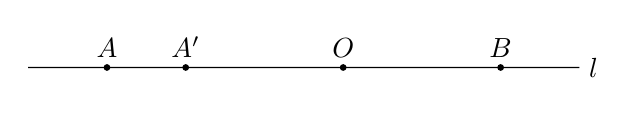
\begin{tikzpicture}
\draw[fill=black] (-3,0)--(-2,0)node[above]{\(A\)}circle(1pt)
--(-1,0)node[above]{\(A'\)}circle(1pt)
--(1,0)node[above]{\(O\)}circle(1pt)
--(3,0)node[above]{\(B\)}circle(1pt)--(4,0)node[right]{\(l\)};
\end{tikzpicture}
\caption{射线}
\label{figure:欧氏几何.射线}
\end{figure}
\end{definition}

\begin{definition}
若干条首尾相连的线段\(AB,BC,CD,\dotsc,KL\)的集合叫做一条\DefineConcept{折线段},
它连结\(A\)和\(L\)这两点.
为求简便,可将这条折线段记为\(ABCD \dotso KL\).
线段\(AB,BC,CD,\dotsc,KL\)的内点和端点都叫做这条折线段的点.
点\(A\)和点\(L\)称为“折线段的\DefineConcept{端点}”.

若折线段\(ABCD \dotso KL\)的顶点\(A,B,C,D,\dotsc,K,L\)都在同一平面上,
且它的端点\(L\)和\(A\)是同一个点,
则这条折线段就叫做一个\DefineConcept{多边形},
记为\(ABCD \dotso K\).
线段\(AB,BC,CD,\dotsc,KA\)叫做“多边形的\DefineConcept{边}”.
点\(A,B,C,D,\dotsc,K\)叫做“多边形的\DefineConcept{顶点}”.

若一个多边形有三个顶点,
则称之为\DefineConcept{三角形}.
设三角形的三个顶点分别为\(A\)、\(B\)、\(C\),
则可将其表记为以下六个符号中的任意一个:
\begin{equation*}
\begin{split}
\triangle ABC, \qquad
\triangle ACB, \qquad
\triangle BAC, \\
\triangle BCA, \qquad
\triangle CAB, \qquad
\triangle CBA.
\end{split}
\end{equation*}

若一个多边形有\(n\ (n>3)\)个顶点,
则称之为\(n\) \DefineConcept{边形}.

若一个多边形的顶点各各不同,
它的任一边内不含有顶点,
且它的任意两边无公共点,
这个多边形就叫做\DefineConcept{简单多边形}.
\end{definition}

根据\cref{theorem:欧氏几何.定理8} 可以推出下列两条推论:
\begin{theorem}\label{theorem:欧氏几何.定理9}
一平面\(\alpha\)上的每一个简单多边形,
把平面\(\alpha\)上其余点%
(即平面\(\alpha\)上的,
而不在这多边形的边上的点)%
分为\DefineConcept{内域}和\DefineConcept{外域}两个区域.
这两个区域具有如下性质:
\begin{enumerate}
	\item 若\(A\)是“内域的一个点(内点)”,
	而且\(B\)是“外域的一个点(外点)”,
	则平面\(\alpha\)上任意一条连接\(A\)和\(B\)的折线段,
	至少和多边形有一公共点.

	\item 若\(A\)和\(C\)是内点,
	而\(B\)和\(D\)是外点,
	则在平面\(\alpha\)上恒有连接\(A\)和\(C\)的折线段,
	和连接\(B\)和\(D\)的折线段,
	它们都和多边形无公共点.

	\item 平面\(\alpha\)上存在全含于外域的直线,
	而不存在全含于内域的直线.
\end{enumerate}
\end{theorem}

\begin{theorem}\label{theorem:欧氏几何.定理10}
每一平面\(\alpha\)把空间中其余点分为具有下述性质的两个区域:
\begin{enumerate}
	\item 一区域的任一点\(A\)和另一区域的任一点\(B\)所决定的线段\(AB\)内,必含有\(\alpha\)的一点.
	\item 同一区域的任意两点\(A\)和\(C\)所决定的线段\(AC\)内,恒不含有\(\alpha\)的点.
\end{enumerate}
\end{theorem}

\begin{definition}
在\cref{theorem:欧氏几何.定理10} 的条件下,
我们说“\(A\)和\(C\)这两点在空间中平面\(\alpha\)的\DefineConcept{同侧}”,
说“\(A\)和\(B\)这两点在空间中平面\(\alpha\)的\DefineConcept{异侧}”.
\end{definition}
